\chapter{OSC Examples}\label{chap:oscexamples}\index{OSC Examples}
The examples provided use the HappyBrackets creative coding toolkit and are coded in Java. For details on installing HappyBrackets, see section \ref{subsec:runningexamples} --
\emph{\titleref{subsec:runningexamples}}

The examples are configured to use port 1234 as the port you will receive OSC from Stellar Command. Additionally, it is configured to have Stellar Command listend on ports 3333, 4444 or 5555. These are the same configuration setting used in the description in section \ref{sec:launchcommand} --
\emph{\titleref{sec:launchcommand}}. Examples of videos showing OSC messages using with Stellar Command can be found at \url{https://www.youtube.com/playlist?list=PLZvzDO0UIKxO-Vlnt30ciKefTcKxupz0n}.

\subsection{Example Source Location}\index{OSC Examples!Example files location}

The source files for the OSC examples are under the \textit{src/stellarcommandexamples/osc} folder, as shown in 
Figure~\ref{fig:oscexamplefolder}.

\begin{figure}[htbp]
	\centering
	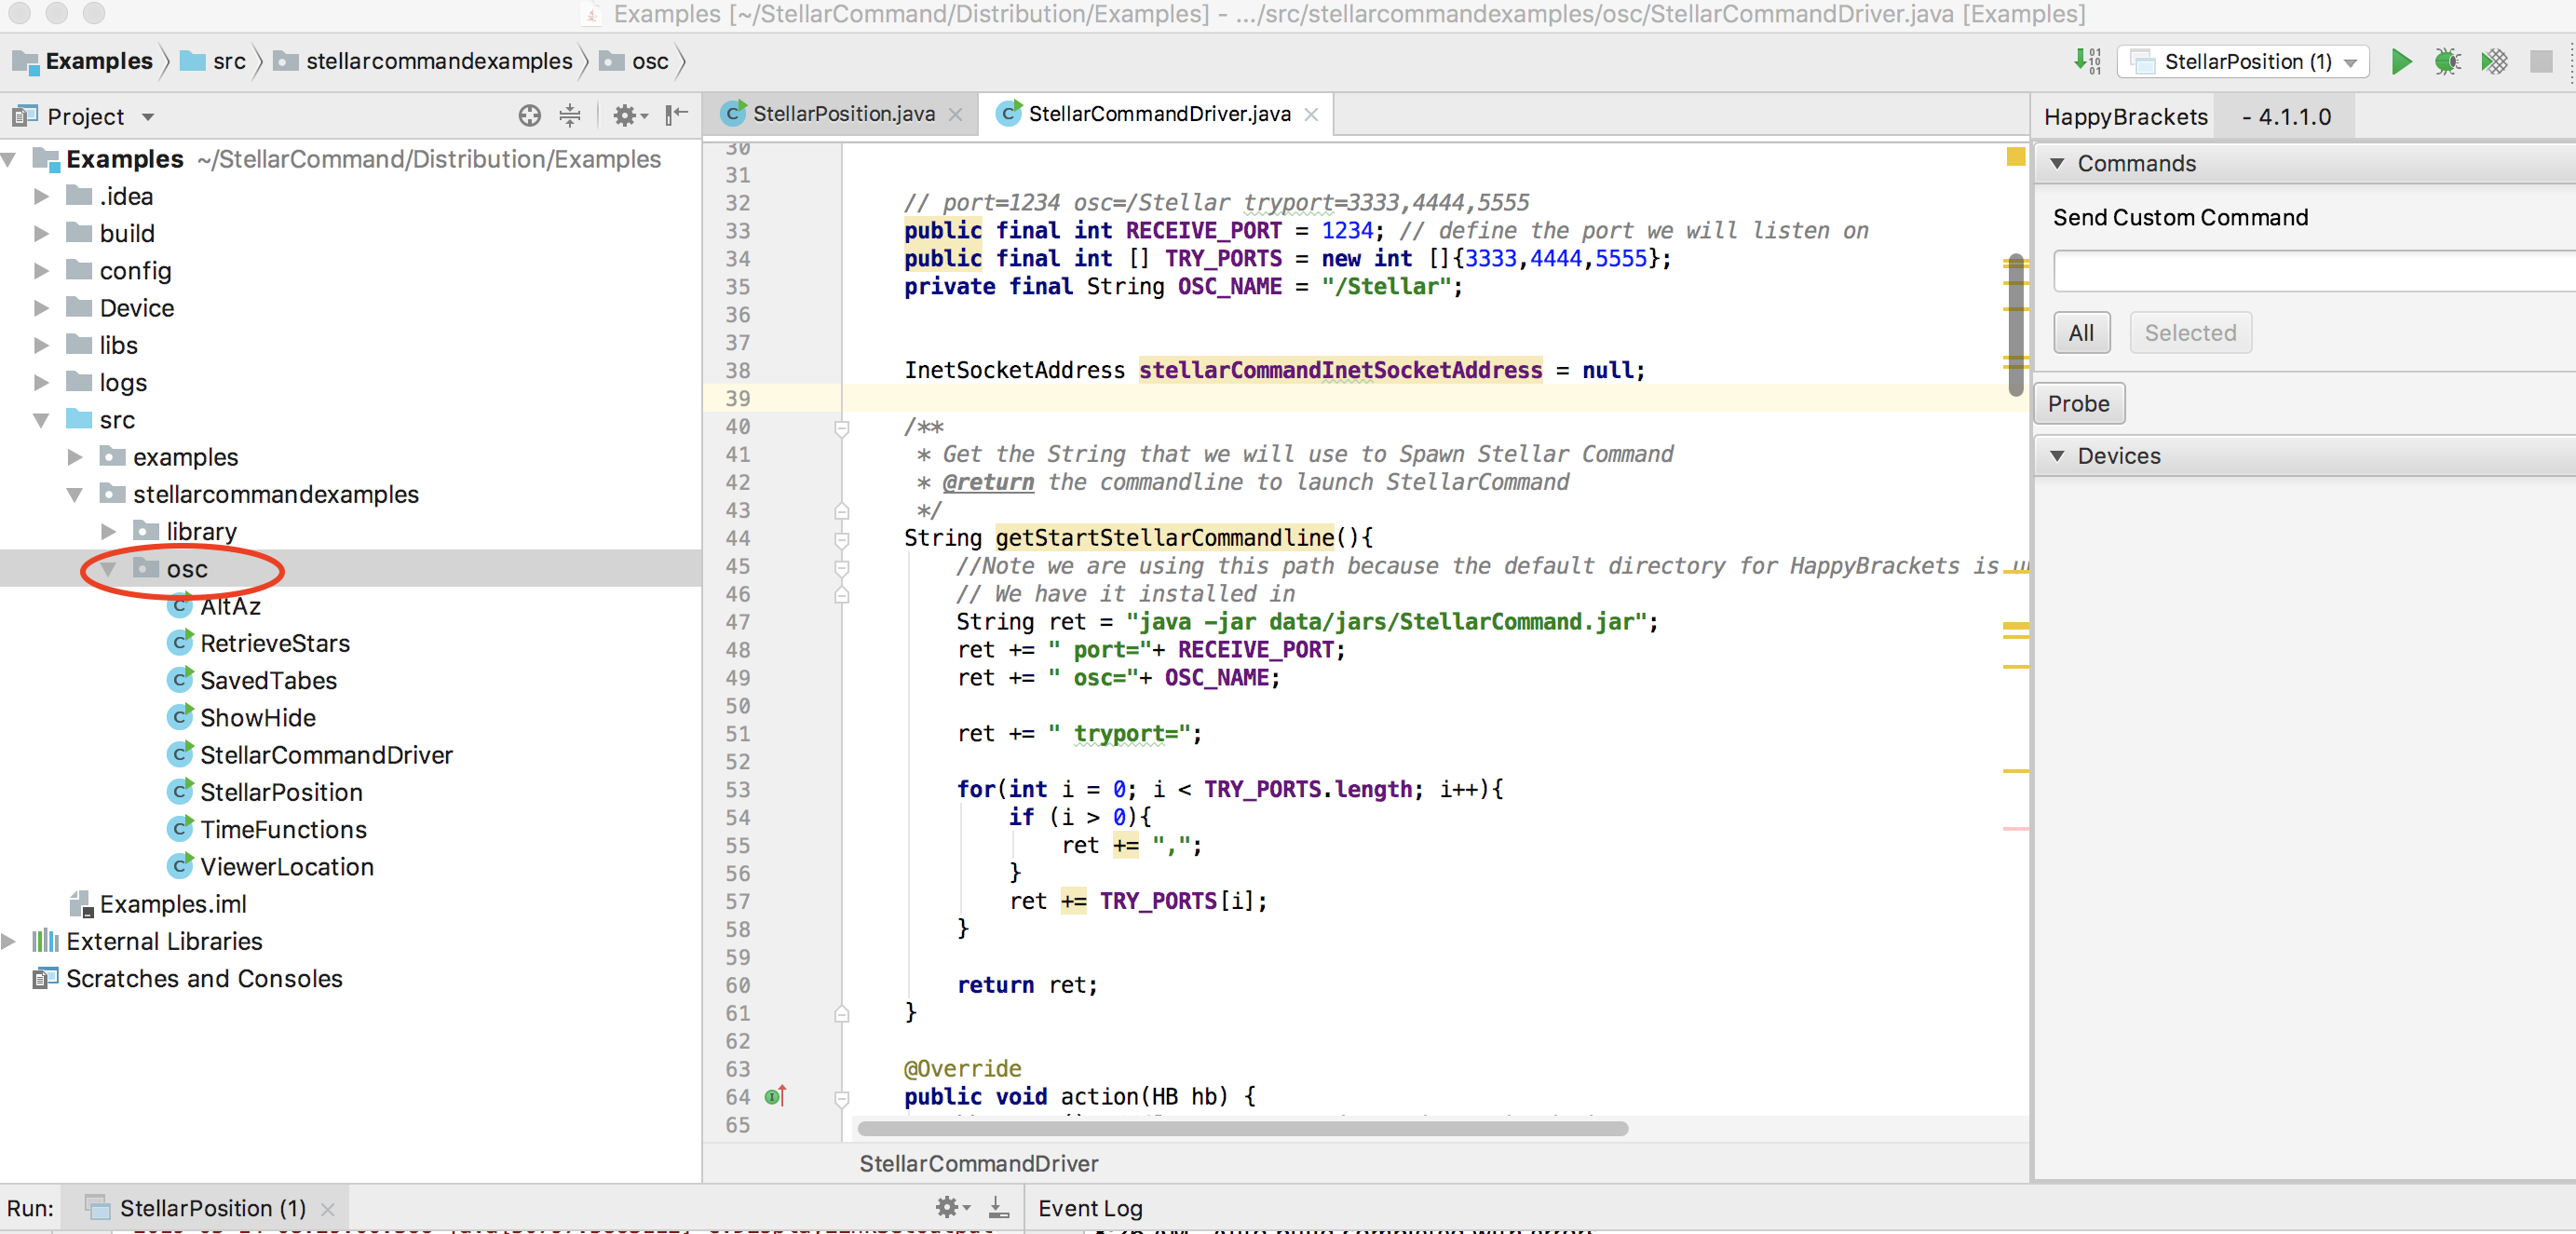
\includegraphics[width=1\columnwidth]{oscexamplefolder}
	\caption{OSC examples folder.}
	\label{fig:oscexamplefolder}
\end{figure}

\subsection{Human Readable OSC Messages}
OSC messages have bee converted to a human readable string through the function \textit{StellarOSCVocabulary.getOscAsText}. This function has been used to facilitate displaying OSC messages in both the send and receive OSC examples.

\subsection{Java Docs} \index{OSC Examples!Java Docs}
Documentation for the examples is effected through Java docs, which can be accessed by pressing the \textit{F1} key. 

\index{OSC Examples!OSC Constants} Often, constants have been used instead of typing literal string values. For example, Figure~\ref{fig:exampleConstantShow} shows the constant \textit{StellarOSCVocabulary.CommandMessages.ALTITUDE} used instead of typing the literal "altitude". 
\begin{figure}[htbp]
	\centering
	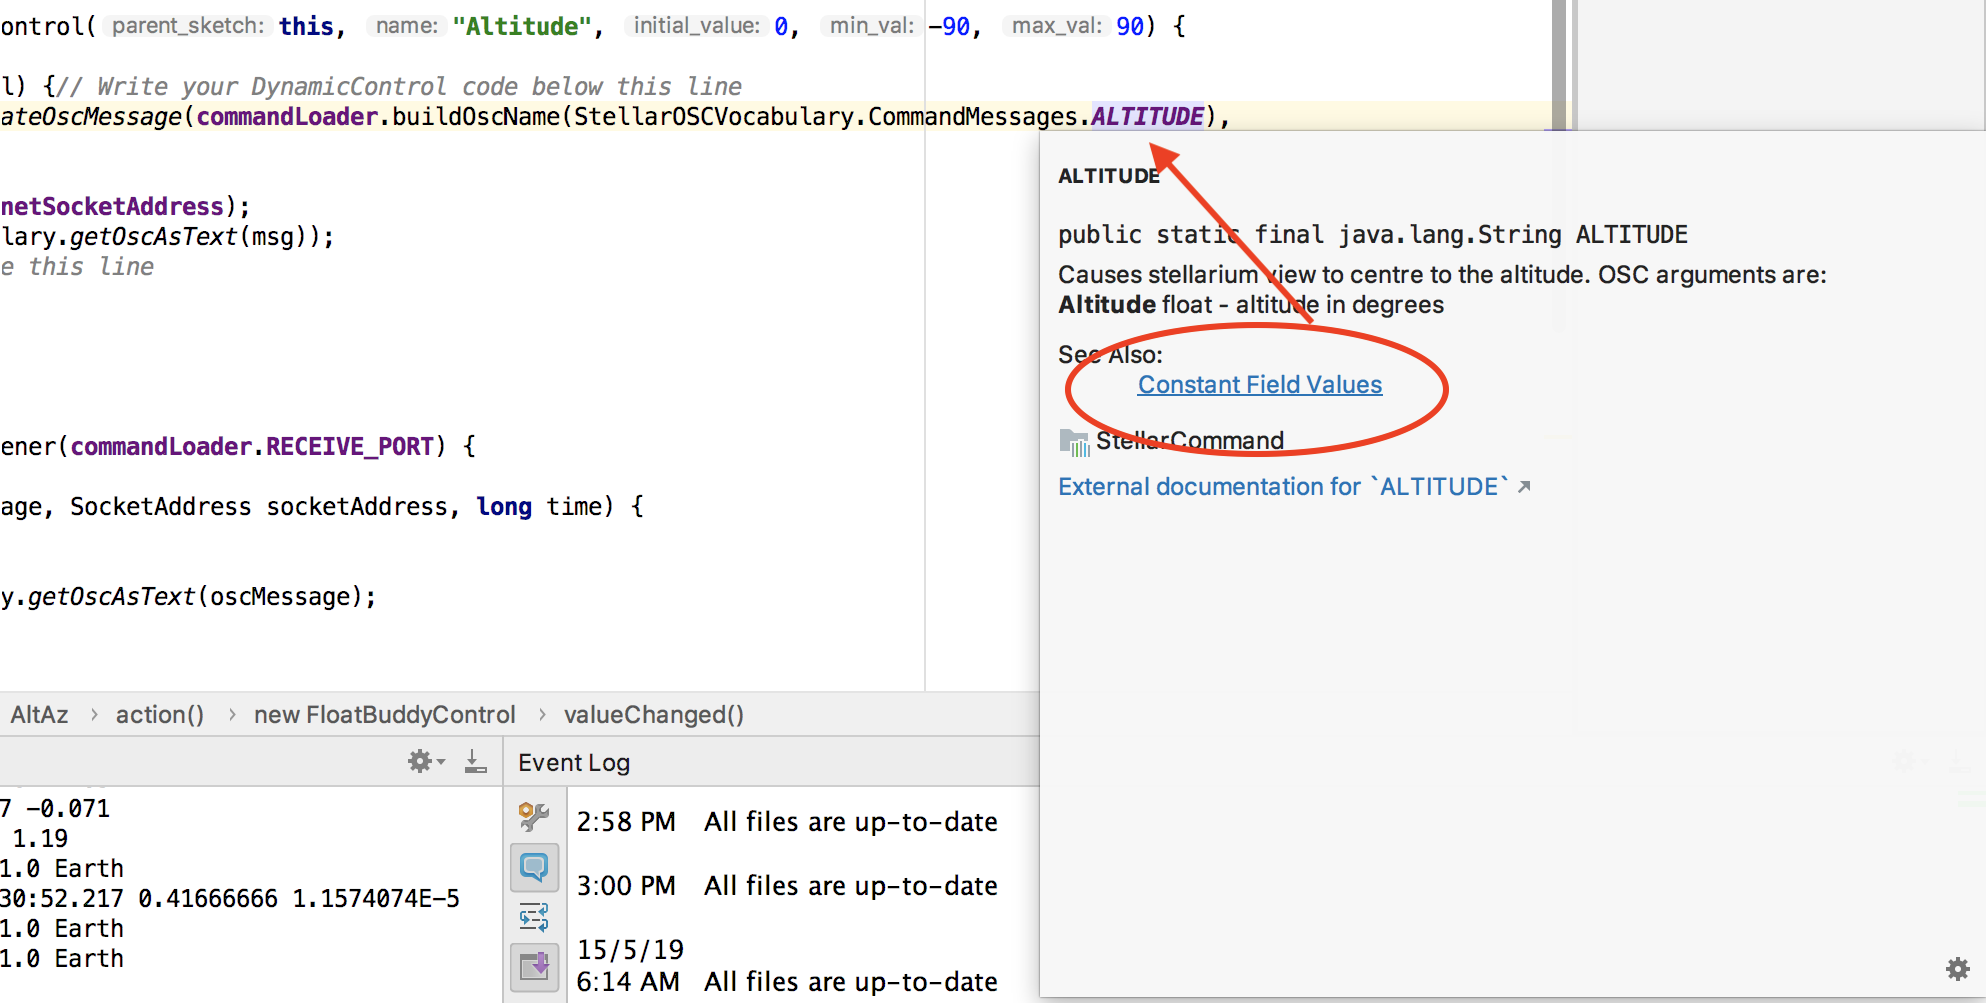
\includegraphics[width=1\columnwidth]{exampleConstantShow}
	\caption{OSC examples folder.}
	\label{fig:exampleConstantShow}
\end{figure}
You can view the value of the constant by selecting it in the editor, pressing the \textit{F1} key and then clicking the \textit{Constant Field Values} link. This will display the Java documentation as shown in Figure~\ref{fig:constantDisplay}.

\begin{figure}[htbp]
	\centering
	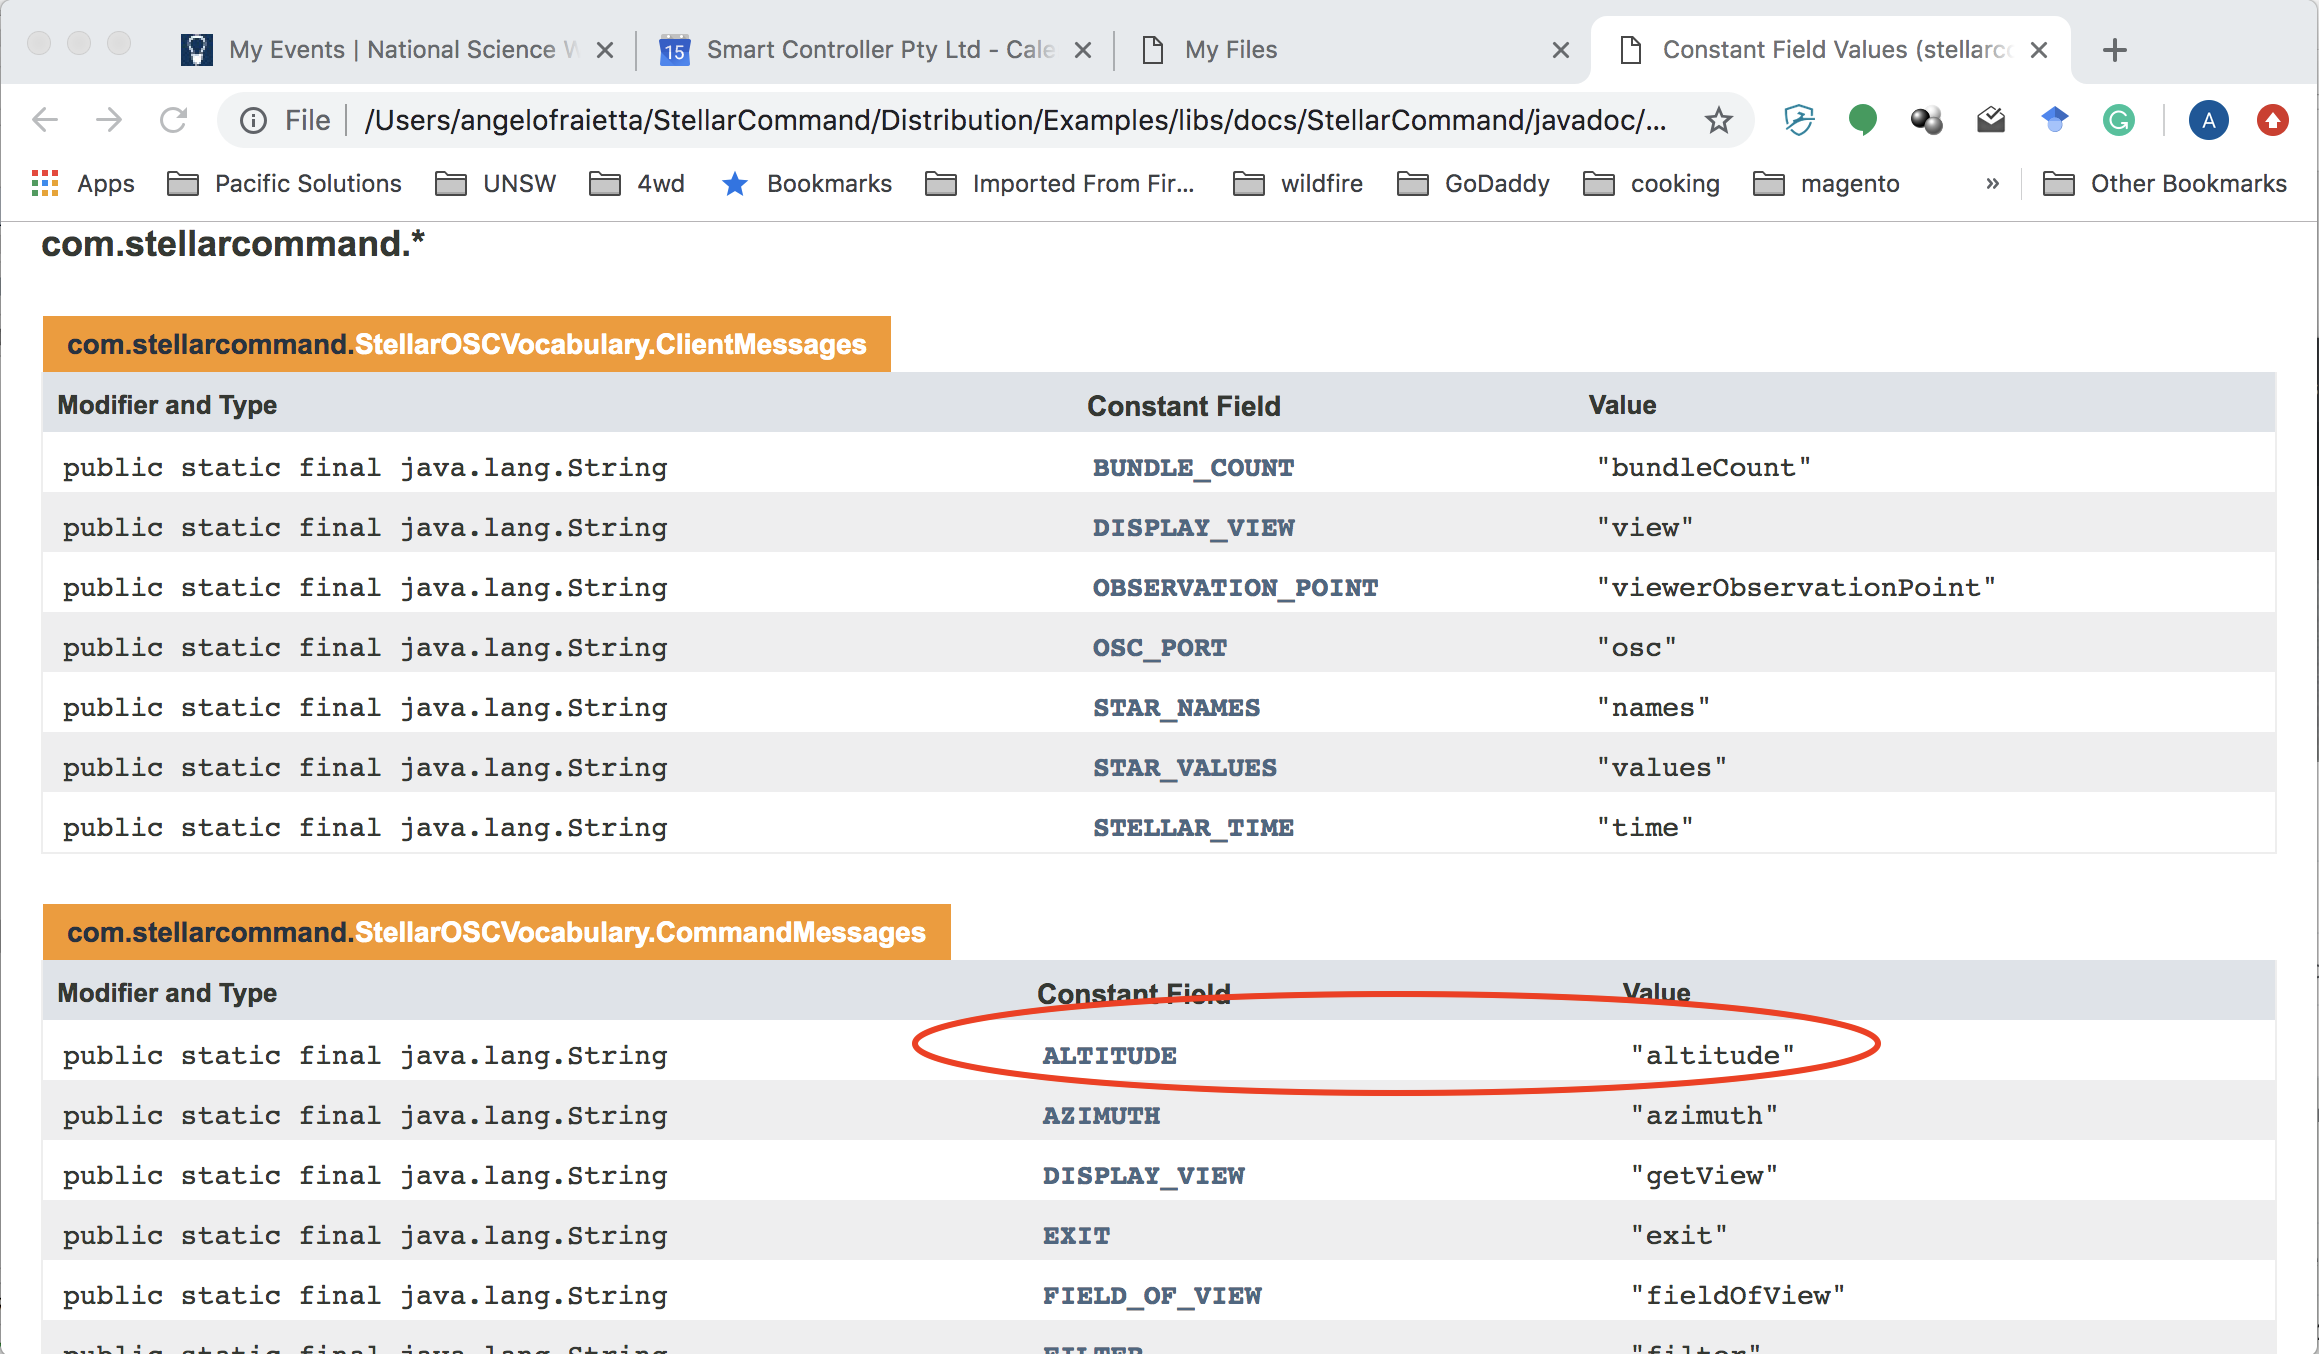
\includegraphics[width=1\columnwidth]{constantDisplay}
	\caption{OSC examples folder.}
	\label{fig:constantDisplay}
\end{figure}

constantDisplay

\section{Sending OSC in Examples}
Some of the examples display sending OSC messages to Stellar Command. 
These examples use HappyBrackets dynamic controls, which are basically text boxes, sliders, checkboxs and buttons, to create OSC messages, which are sent to Stellar Command. For example, Figure~\ref{fig:exampleAzimuth} shows the \textit{AltAz} example for changing the altitude and azimuth. In the image, the azimuth is being changed by the controls in the red box, which call the function \textit{valueChanged}. The OSC message is packed and sent to Stellar Command using the functions \textit{commandLoader.buildOscName} and  \textit{OSCMessageBuilder.createOscMessage}.\index{OSC messages to Stellar Command!azimuth}  The actual OSC message contents, however, are displayed in the \textit{Diagnostics} text box so you can see what the actual OSC message sent is, which in the case of the Figure~\ref{fig:exampleAzimuth} is \textit{/Stellar/azimuth 35.064934}
 \footnote{See \ref{subsec:azimuth} --
 	\emph{\titleref{subsec:azimuth}} for details of this message.}.
 All the examples will display the OSC message sent in the diagnostic window.  

\begin{figure}[htbp]
	\centering
	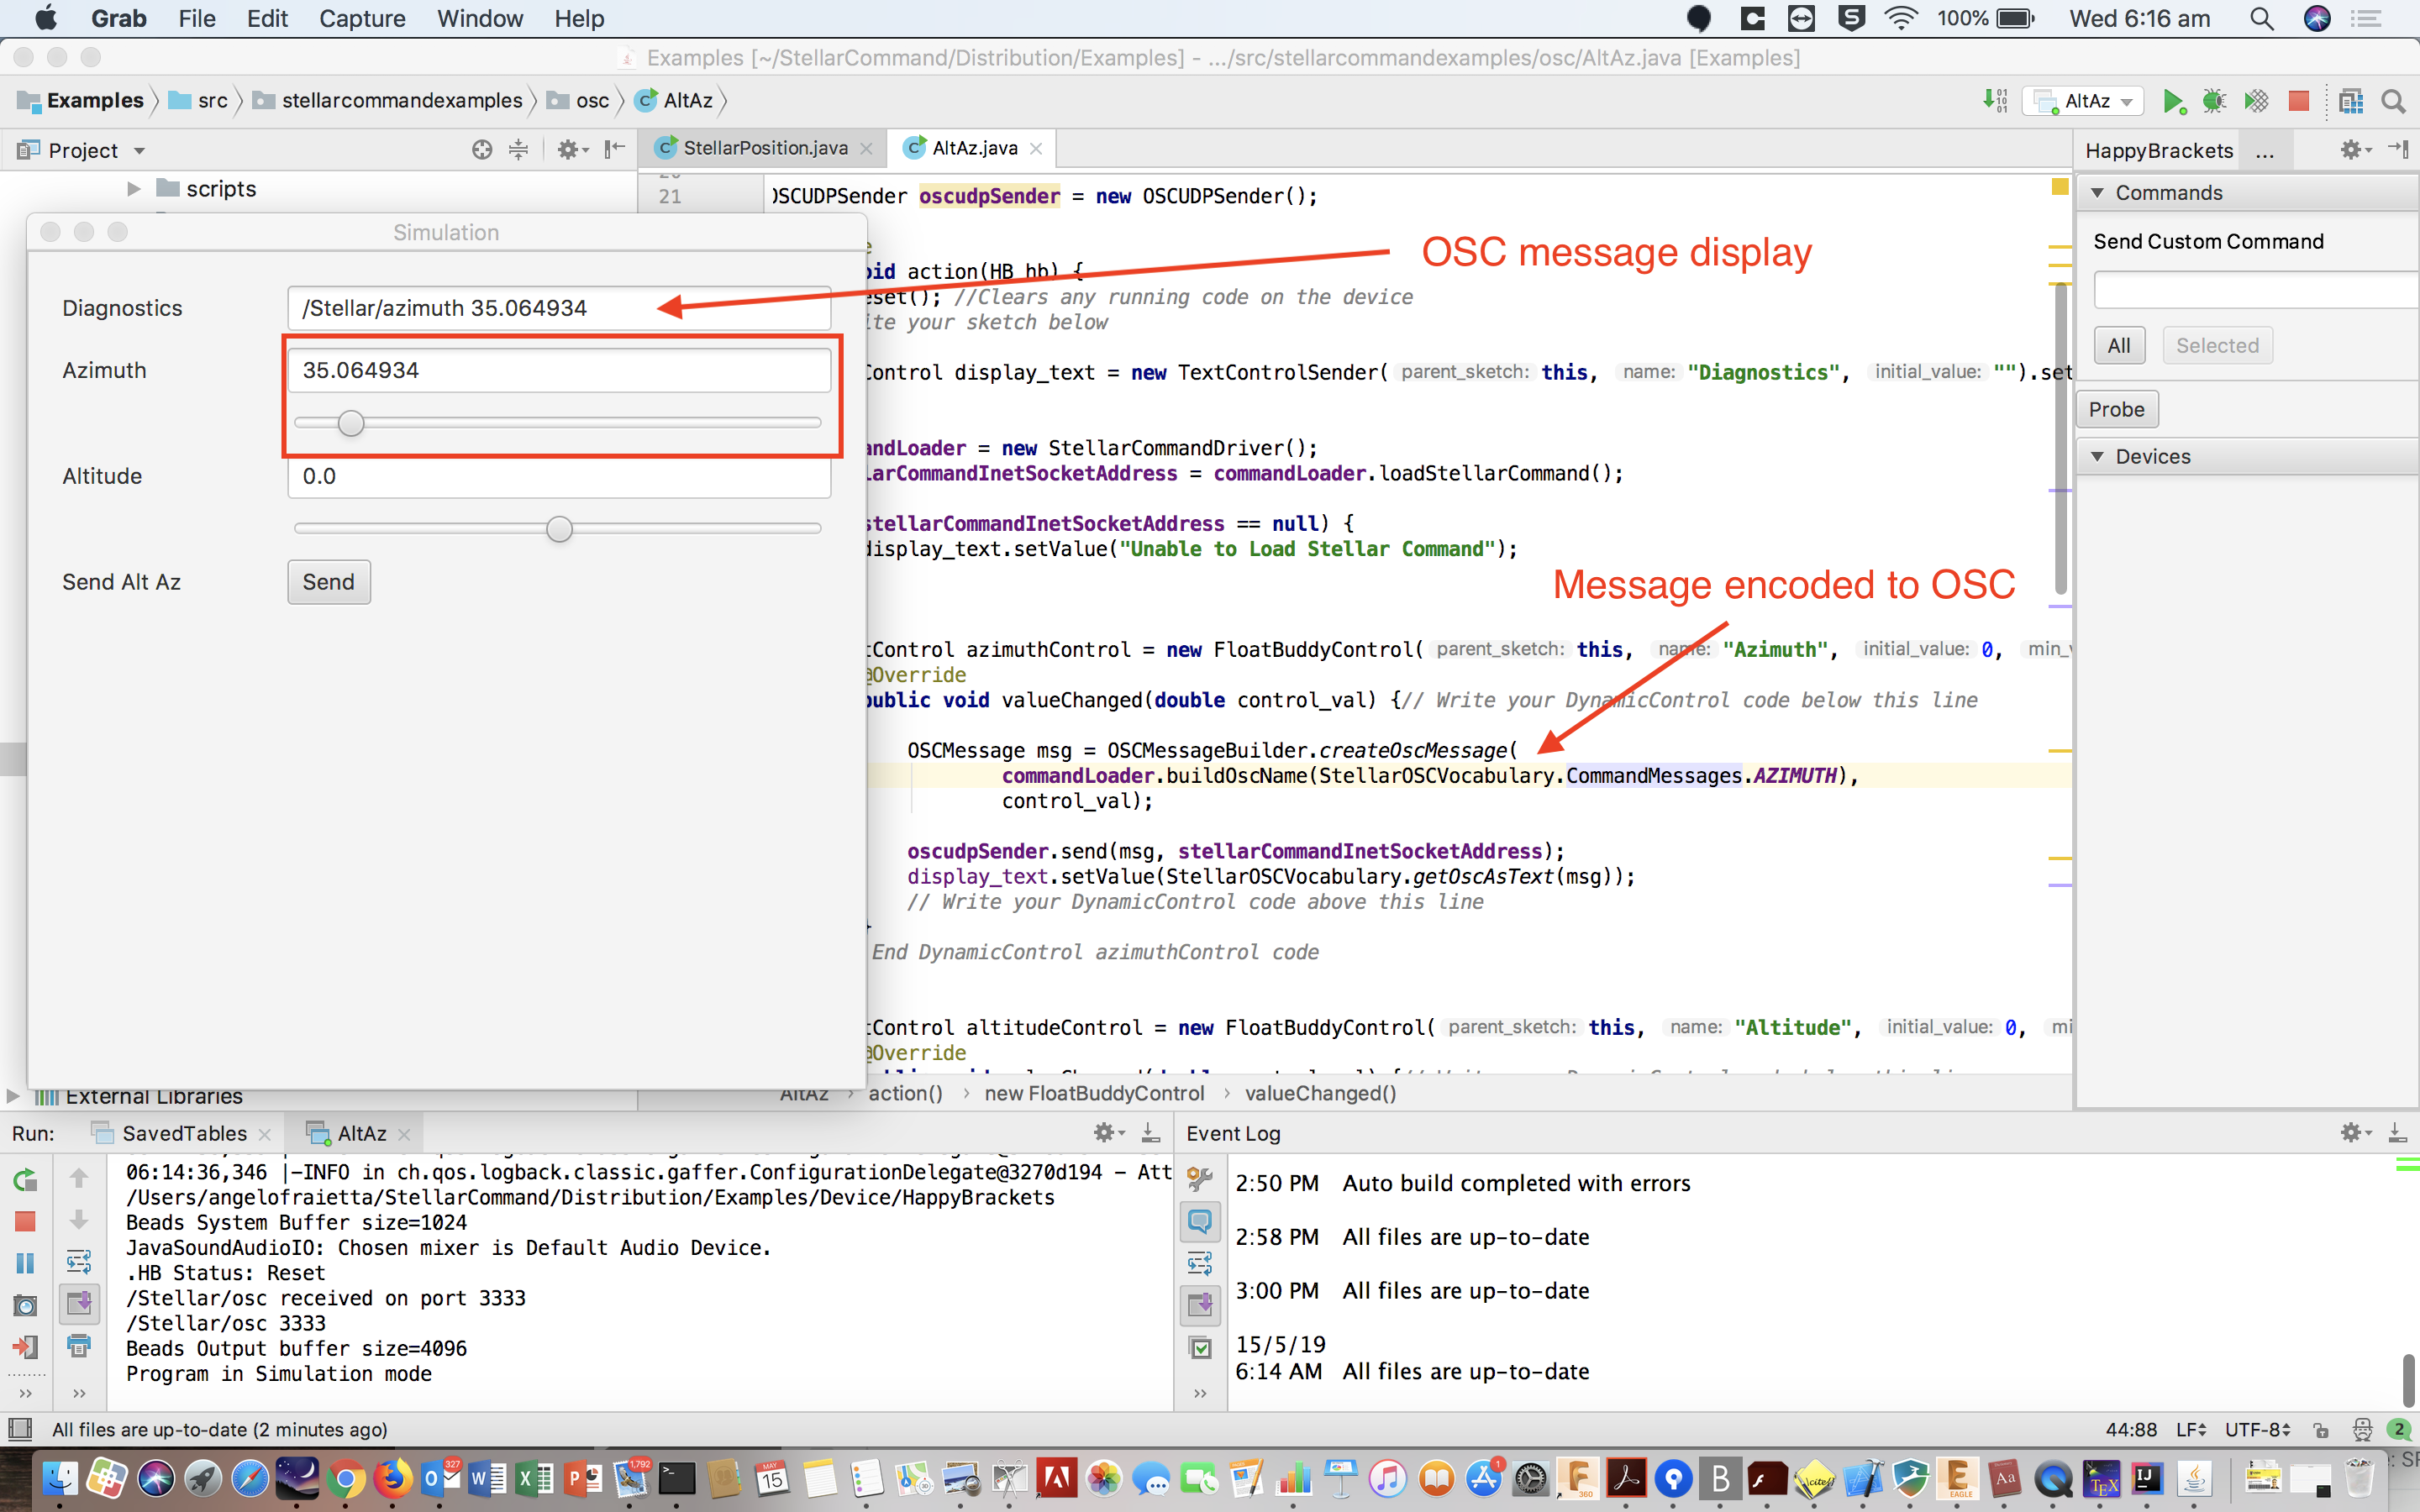
\includegraphics[width=1\columnwidth]{exampleAzimuth}
	\caption{AltAz example.}
	\label{fig:exampleAzimuth}
\end{figure}


\section{Receiving OSC in Examples}\label{sec:oscreceiveexample}
Some of the examples display OSC messages that have been received from Stellar Command. For example, Figure~\ref{fig:oscExampleReceive} shows  OSC received through the \textit{OSCReceived} function. The OSC message is decoded and displayed in the IntelliJ console output, shown inside the red box. 

\begin{figure}[htbp]
	\centering
	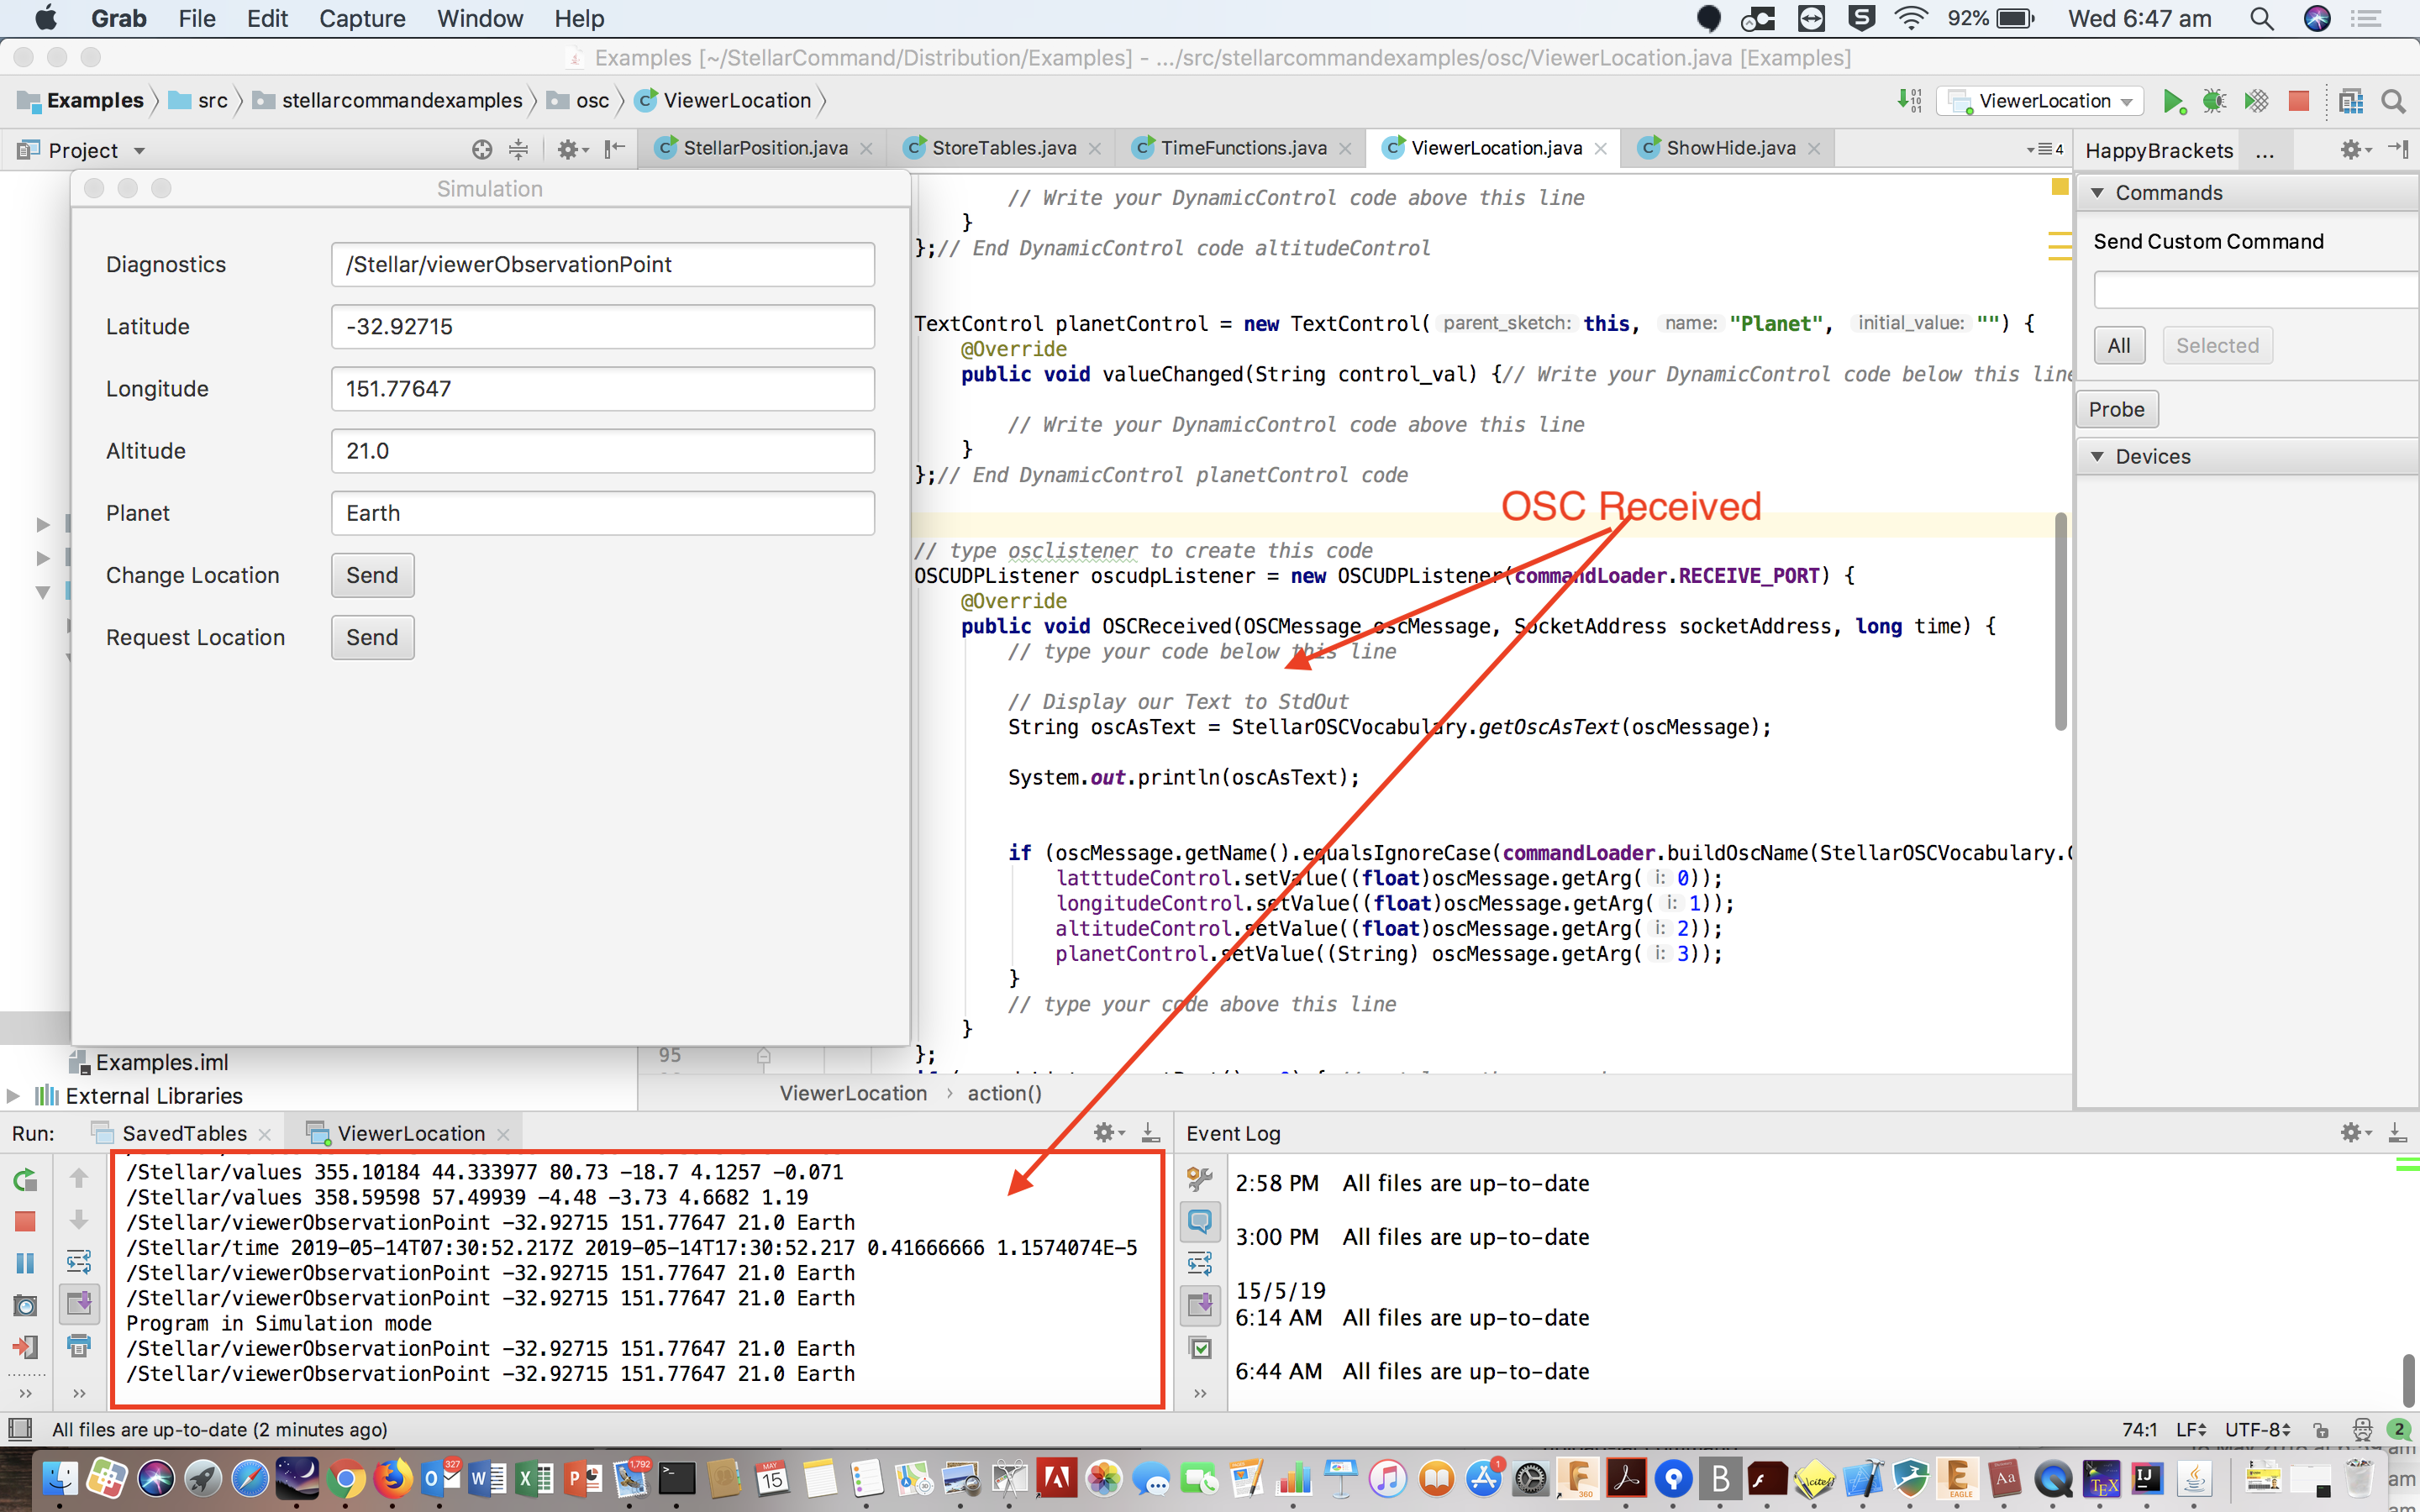
\includegraphics[width=1\columnwidth]{oscExampleReceive}
	\caption{View Observation Point Example.}
	\label{fig:oscExampleReceive}
\end{figure}

Bundles are separated in the examples, with each message in the bundle processed in sequence, as shown in Figure~\ref{fig:exampleStellar}.

\begin{figure}[htbp]
	\centering
	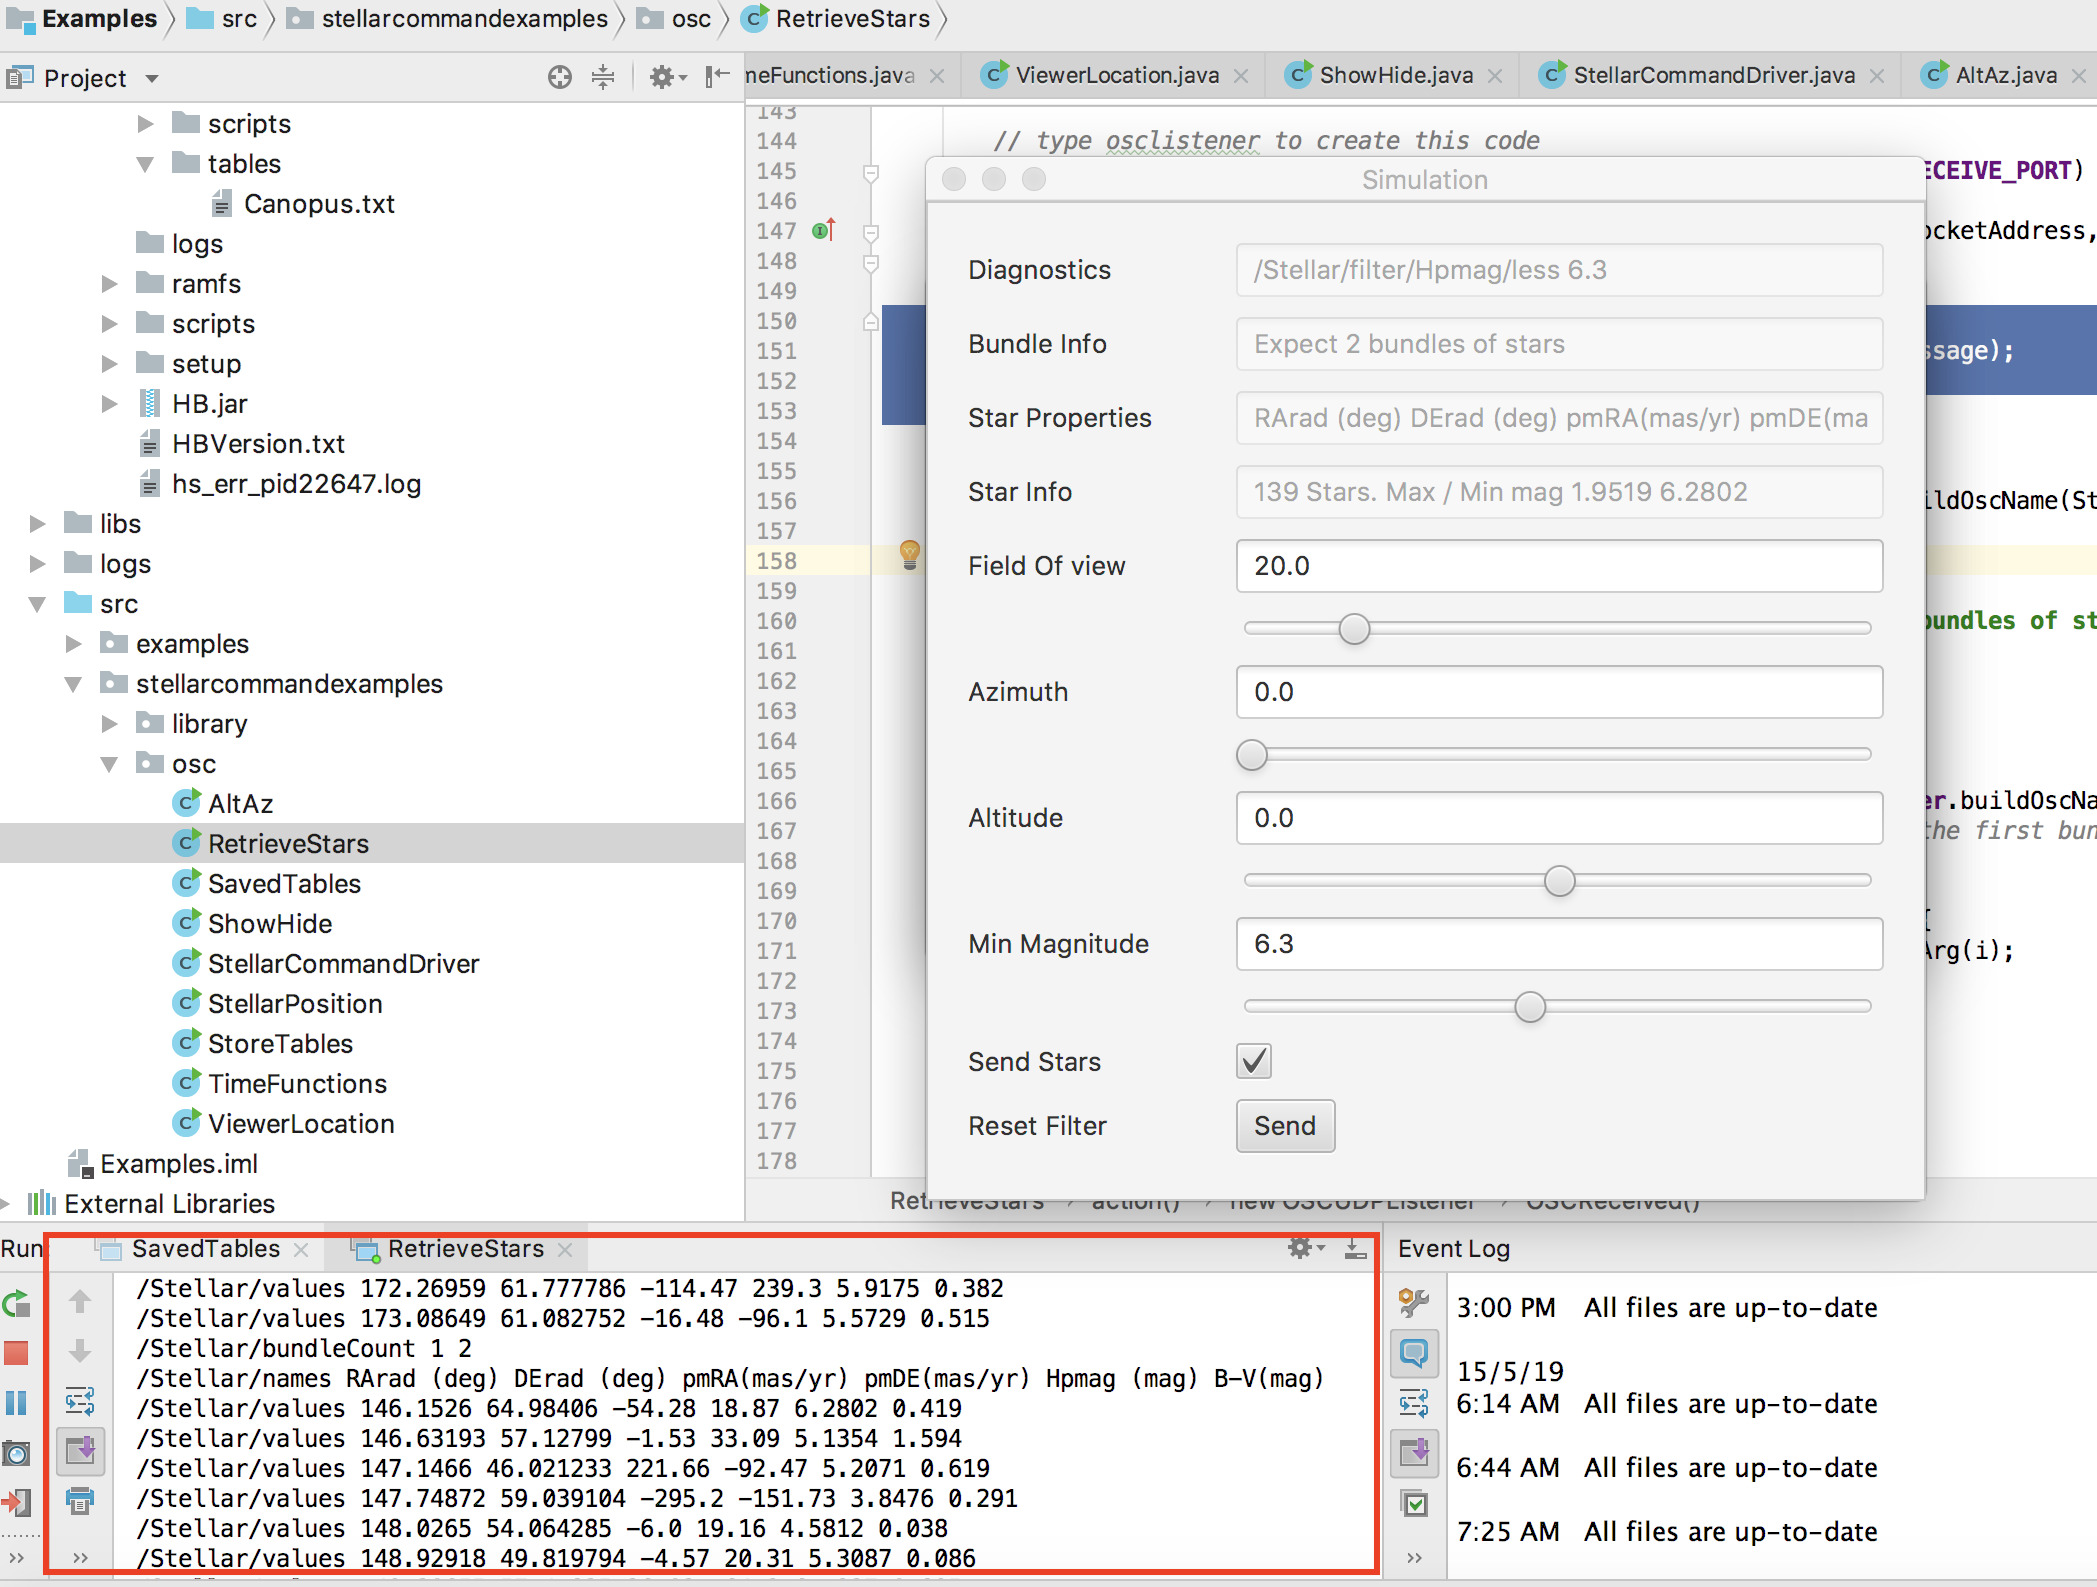
\includegraphics[width=1\columnwidth]{exampleStellar}
	\caption{Receiving Stellar Data Example.}
	\label{fig:exampleStellar}
\end{figure}


